\section{Zielsetzung}
\label{sec:Zielsetzung}
Es soll mittels Doppler-Sonographie die Fließgeschwindigkeit und das Strömungsprofil an Strömungsrohren
untersucht werden.

\section{Theorie}
\label{sec:Theorie}
Allgemein sind Schallwellen im Frequenzbereich von $\SI{16}{\kilo\hertz}$ bis $\SI{20}{\kilo\hertz}$ hörbar.
Der Frequenzbereich von $\SI{20}{\kilo\hertz}$ bis $\SI{1}{\giga\hertz}$ wird Ultraschall genannt. Der
Frequenzbereich darüber wird Hyperschall genannt. Durch Aussenden durch eine Ultraschallsonde und anschließende
Reflexion am Material können so die Eigenschaften des Materials bestimmt werden. Der Ultraschall wird in der Sonde
durch Quarz-Kristalle mit Hilfe des Piezoelektrischen Effekts erzeugt. Der Piezoelektrische Effekt sorgt bei einer
Anregung durch ein äußeres E-Feld für die Emission von Ultraschall. Durch den reziproken Piezoelektrischen
Effekt können die reflektierten Ultraschallwellen ausgewertet werden.\\
Um die Geschwindigkeit eines Teilchens in einer Flüssigkeit zu bestimmen, wird der Dopplereffekt ausgenutzt.
Der Dopplereffekt sorgt dafür, dass bei relativer Geschwindigkeit ziwschen Quelle und Empfänger eine
Frequenzverschiebung auftritt. Bewegen sich Quelle und Beobachter voneinander weg wird die Frequenz
$\nu_{\symup{0}}$ zu einer niedrigeren Frequenz $\nu_{n}$ verschoben. Dies lässt sich durch
\begin{equation}
    \label{dopplern}
    \nu_{\symup{h/n}} = \frac{\nu_{\symup{0}}}{1\mp \frac{v}{c}}
\end{equation}
asudrücken.
Bewegen sich Quelle und Beobachter aufeinander zu wird die Frequenz zu einer höheren Frequenz $\nu_{h}$ verschoben.
Dies lässt sich durch 
\begin{equation}
    \label{eqn:dopplerh}
    \nu_{\symup{h/n}} = \nu_{\symup{0}}\left(1 \pm \frac{v}{c}\right)
\end{equation}
beschreiben. Dabei sind $v$ die Geschwindigkeit des Objekts und $c$ die Ausbreitungsgeschwindigkeit im Material.
Wird nun eine strömende Flüssigkeit mit einzelene Festkörpern untersucht, lässt sich aus den in
\autoref{fig:stroemung} geometrischen Überlegung die Frequenzverschiebung durch
\begin{equation}
    \label{eqn:fdiff}
    \Delta \nu = 2\nu_{\symup{0}}\frac{v}{c}\cos(\alpha)
\end{equation}
bestimmen. Dabei ist $\alpha$ der Winkel zwischen der Geschwindigkeit $v$ und der Wellennormalen.
\begin{figure}
    \centering
    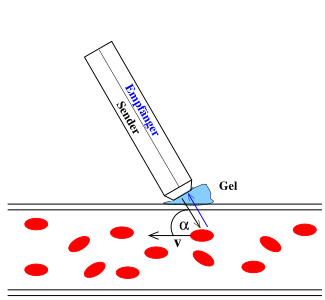
\includegraphics{Bilder/stroemung.png}
    \caption{Schematische Darstellung der Doppler-Sonographie an einem Blutgefäß \cite{sample}.}
    \label{fig:stroemung}
\end{figure}
In der Praxis werden sogenannte Doppler-Prismen verwendet, die bei unterschiedlichen Winkeln für gleichbleibende
Bedingungen sorgen. Für das in \autoref{fig:prisma} dargestellte Prisma lässt sich für $\alpha$ der Zusammenhang
\begin{equation}
    \label{eqn:alpha}
    \alpha = 90^{\circ} - \arcsin(\sin{\theta}\cdot \frac{c_{\symup{L}}}{c_{\symup{P}}})
\end{equation}
mit dem Prismenwinkel $\theta$, der Geschwindigkeit der Dopplerflüssigkeit $c_{\symup{L}}$ und
der Geschwindigkeit des Prismas $c_{\symup{P}}$ bestimmen.
\begin{figure}
    \centering
    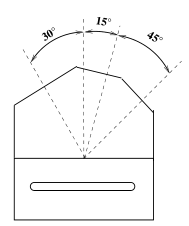
\includegraphics{Bilder/prisma.png}
    \caption{Darstellung des im Versuch verwendeten Doppler Primas \cite{sample}.}
    \label{fig:prisma}
\end{figure}